%====================================================================================
\section[Robinson Crusoe]{Economía Robinson Crusoe: Análisis de Pareto}
%====================================================================================

\begin{frame}{Un modelo sencillo}
Un agente se comporta simultáneamente como consumidor y como productor.
	\begin{itemize}
		\item En esta economía competitiva tendremos:
		\item Una empresa que, a la vista de los precios de los factores y de los productos, decide contratar una cierta cantidad de horas de trabajo con el objetivo de producir un bien de consumo y maximizar su beneficio;
		\item un Robinson trabajador que vende horas de su ocio a la empresa en forma de trabajo y recibe un salario;
		\item un Robinson empresario que recibe el beneficio; y
		\item un Robinson consumidor que decide comprar una canasta de bienes (ocio, bien de consumo) a la empresa con el objetivo de maximizar su satisfacción.
	\end{itemize}
\end{frame}
%-------------------------------------------------
\begin{frame}{Un modelo sencillo}
		\begin{itemize}
			\item Preferencias de Robinson:
						$$u(c,R)=u(c,\overline{L}-L)$$
					$c:$ cantidad consumida del bien, $R:$ cantidad consumida del bien, $\overline{L}:$ Dotación de tiempo y $L:$ horas ofrecidas de trabajo.
			\item Tecnología
						$$q=f(L)$$
					$q:$ Cantidad producida del bien y $L:$ horas demandadas de trabajo.
		\end{itemize}
\end{frame}
%-------------------------------------------------
\begin{frame}{Un modelo sencillo}
	El modelo se subdivide en los siguientes problemas:
		\begin{enumerate}
			\item Asignación eficiente.
			\item El problema de la empresa.
			\item El problema del consumidor.
		\end{enumerate}
\end{frame}
%-------------------------------------------------
\begin{frame}{Asignación eficiente}
	Objetivo: identificar la combinación $(L,q)$ consistente con la dotación de tiempo y la tecnología que maximice $u(c,R)$.
		\begin{align*}
			& \text{Max } \quad u\left(c,R\right) \\
			& \begin{array}{ll}
				\text{s.a: } & c = q = f(L) \\[0.1cm]
							 & R = \overline{L}- l
			\end{array}
		\end{align*}
	En el óptimo: $RMS = PMg_L$\\
		\begin{center}
			\begin{tikzpicture}[domain=5:10,
					tangent/.style={
						decoration={
							markings,% switch on markings
							mark=
							at position #1
							with
							{
								\coordinate (tangent point-\pgfkeysvalueof{/pgf/decoration/mark info/sequence number}) at (0pt,0pt);
								\coordinate (tangent unit vector-\pgfkeysvalueof{/pgf/decoration/mark info/sequence number}) at (1,0pt);
								\coordinate (tangent orthogonal unit vector-\pgfkeysvalueof{/pgf/decoration/mark info/sequence number}) at (0pt,1);
							}
						},
						postaction=decorate
					},
					use tangent/.style={
						shift=(tangent point-#1),
						x=(tangent unit vector-#1),
						y=(tangent orthogonal unit vector-#1)
					},
					use tangent/.default=1,
					scale=0.65
					]
	% Relleno
		\fill [pattern=crosshatch dots,pattern color=orange!60!white] (5,5) -- plot (\x, {sqrt(10-\x)/0.5 }) -- (5,0);\textbf{}
	% Ejes
		% Izquierda
			\draw[<->] (4,0) node[align=center, left, scale=0.8] {$-L$} -- (10,0) node[align=center, below] {\footnotesize $O_L$} -- (10,5) node[align=center, above, scale=0.8] {$q$};
		% Derecha
			\draw[<->] (5,5) node[align=center, above, scale=0.8] {$c$} -- (5,0) node[align=center, below, scale=0.8] {$O_R$} -- (11,0) node[align=center, right, scale=0.8] {$R$};
	% Curva
		\draw[color=orange,samples=1000, tangent=0.4] plot (\x, {sqrt(10-\x)/0.5 });
	% Punto - Tangente
		\filldraw[use tangent] (0,0) circle (2pt) node[align=center, above right, scale=0.8] {$M$};
	% Flechas
		\draw[<->] (5,-0.5) -- (7.5,-0.5) node[align=center, below, scale=0.8] {$\overline{L}$} -- (10,-0.5);
	% Curvas de indiferencia
		\draw [smooth,blue,thick] (6.3,5.5) to[out=299, in=161] (10.3,2.7);    
		\draw [smooth,blue,thick] (5.8,5) to[out=299, in=161] (9.8,2.2);
		\draw [smooth,blue,thick] (5.3,4.5) to[out=299, in=161] (9.3,1.7);
\end{tikzpicture}
		\end{center}
\end{frame}
%-------------------------------------------------
\begin{frame}{El problema de la empresa}
	Se introduce el mecanismo de mercado. El empresario Robinson debe decidir la cantidad de trabajo a utilizar para maximizar el beneficio, dados los precios de un bien $(p)$ y mano de obra $(w)$.
			\medskip
		$$\pi = pq - wl$$
			\medskip
	En el óptimo: $PMg_L=\frac{w}{p}$\\
			\vspace{-0.3cm}
		\begin{center}
			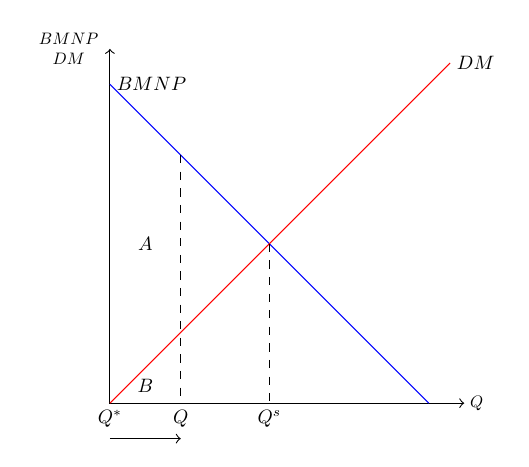
\begin{tikzpicture}[scale=0.9]
% Ejes
\draw[<->] (0,5)  node [text width=15mm,text centered, scale=0.6, left] {$BMNP$ $DM$}-- (0,0) -- (5,0) node [scale=0.6, right] {$Q$};

% Rectas
\draw[blue] (0,4.5) node [right, scale=0.7, black] {$BMNP$} -- (4.5,0);
\draw[red] (0,0)  node [below, scale=0.7, black] {$Q^\ast$} -- (4.8,4.8) node [right, scale=0.7, black] {$DM$};

% Rectas sombreadas
\draw[dashed] (1,3.5) -- (1,0)  node [below, scale=0.7, black] {$Q$};
\draw[dashed] (2.25, 2.25) -- (2.25,0) node [below, scale=0.7, black] {$Q^s$};

% A y B
\draw (0.5,2.25) node [scale=0.7, black] {$A$};
\draw (0.5,0.25) node [scale=0.7, black] {$B$};

% Flechas
\draw[->] (0,-0.5) -- (1,-0.5);
\end{tikzpicture}
		\end{center}
\end{frame}
%-------------------------------------------------
\begin{frame}{El problema del consumidor}
	El ingreso de Robinson consumidor está compuesto de la venta del ocio en forma de trabajo y del beneficio de la empresa.
	$$Y = w(\overline{L}-R)+\pi(p,w)$$
	El problema será:
		\begin{align*}
			& \text{Max } \quad u\left(c,R\right) \\
			& \begin{array}{ll}
				\text{s.a: } & pc \leq w(\overline{L}-R)+\pi(p,w)
			  \end{array}
		\end{align*}
	En el óptimo: $RMS=\frac{w}{p}$\\
			\vspace{2.4cm}
		\begin{center}
			\hspace{-9cm} \begin{tikzpicture}[domain=5:10,
	tangent/.style={
		decoration={
			markings,% switch on markings
			mark=
			at position #1
			with
			{
				\coordinate (tangent point-\pgfkeysvalueof{/pgf/decoration/mark info/sequence number}) at (0pt,0pt);
				\coordinate (tangent unit vector-\pgfkeysvalueof{/pgf/decoration/mark info/sequence number}) at (1,0pt);
				\coordinate (tangent orthogonal unit vector-\pgfkeysvalueof{/pgf/decoration/mark info/sequence number}) at (0pt,1);
			}
		},
		postaction=decorate
	},
	use tangent/.style={
		shift=(tangent point-#1),
		x=(tangent unit vector-#1),
		y=(tangent orthogonal unit vector-#1)
	},
	use tangent/.default=1,
	transform canvas={scale=0.5}
	]       
	% Curva
	\draw[white, samples=1000, tangent=0.4] plot (\x, {sqrt(10-\x)/0.5 });
	% Relleno
	\fill [pattern=crosshatch dots,pattern color=green!60!white] (5,4.74) -- (10,1.6) -- (10,0) -- (5,0) -- (5,6);
	% Ejes
	\draw[<->] (4,0) node[align=center, left, scale=0.8] {$-L$} -- (10,0) node[align=center, below] {\footnotesize $O_L$} -- (10,5) node[align=center, above, scale=0.8] {$q$};
	\draw[<->] (5,5) node[align=center, above, scale=0.8] {$c$} -- (5,0) node[align=center, below, scale=0.8] {$O_R$} -- (11,0) node[align=center, right, scale=0.8] {$R$};
	% Tangente - Punto
	\draw[use tangent] (-2.92,0) -- (4,0);
	\filldraw[use tangent] (0,0) circle (2pt) node[align=center, above right, scale=0.8] {$M$};
	% Flechas
	\draw[<->] (5,-0.5) -- (7.5,-0.5) node[align=center, below, scale=0.8] {$\overline{L}$} -- (10,-0.5);
	% Curvas de indiferencia
	\draw [smooth,blue,thick] (5.8,5) to[out=299, in=161] (9.8,2.2);
	% Linea punteadas
	\draw[dashed] (7.48,0) node [scale=0.8, below] {$R(p,w)$} -- (7.48,3.18) -- (5,3.18) node [scale=0.8, left] {$c(p,w)$};
	% Felcha
	\draw[->] (10.5,2.1) node [scale=0.8, right] {$\frac{\pi(p,w)}{p}$} -- (10,1.6);
	% Etiqueta de pendiente
	\draw (10.9,0.9) node [scale=0.8, right] {$m = \frac{w}{p}$};
	
\end{tikzpicture}
		\end{center}
\end{frame}
%-------------------------------------------------
\begin{frame}{Equilibrio Walrasiano}
	En consecuencia, en equilibrio walrasiano, a los precios $(p^*,w^*)$ tanto el mercado de trabajo como el bien de consumo están equilibrados:
		\begin{gather*}
			\text{Oferta del bien = demanda del bien} \qquad q(p^*,w^*) = c(p^*,w*)\\
			\text{Oferta de trabajo = demanda de trabajo} \qquad \overline{L} - R(p^*,w^*) = L(p*,w*)
		\end{gather*}
	
	\begin{itemize}
		\item 	Una combinación (consumo, ocio) puede surgir como equilibrio competitivo sss maximiza la utilidad del consumidor sujeto a las restricciones impuestas por la tecnologìa y la disponibilidad de recursos.
		\item Una asignación walrasiana es la misma asignación que se hubiera obtenido si un planificador central gestionara la economía con el objetivo de maximizar el bienestar del consumidor.
	\end{itemize}
\end{frame}
%-------------------------------------------------
\begin{frame}{Equilibrio Walrasiano}
	La solución conjunta al modelo de la Economía Robinson Crusoe.\\
		\begin{center}
			\begin{tikzpicture}
	% Formato de CAJA
	\draw[->] (0.5,0.5) node[align=center, below left] {\footnotesize $O_A$} -- (0.5,4.5) node[align=center, above] {\footnotesize $x_{2}^{A}$};
	\draw[->] (0.5,0.5) -- (8.5,0.5) node[align=center, right] {\footnotesize $x_{1}^{A}$};
	
	\draw[->] (8,4) node[align=center, above right] {\footnotesize $O_B$} -- (0,4) node[align=center, left] {\footnotesize $x_{2}^{B}$};
	\draw[->] (8,4) -- (8,0) node[align=center, below] {\footnotesize $x_{2}^{B}$};
	
	% Curvas de indiferencia1
		% Agente A1
			\draw [blue] (1.51,3.5) --  (1.51,1.14) -- (4.01,1.14);
			\draw [blue] (2.82,3.5) -- (2.82,1.98) --  (4.4,1.98);
			\draw [blue] (4.28,3.5) --  (4.28,2.91) -- (4.9,2.91);
			
		% Agente B
			\draw  [red] (0.6,1.5) ..controls (1.4,1.4) and (1.74,1) .. (2,0.55);
			\draw  [red] (1.6,2.5) ..controls (2.4,2.4) and (3,2) .. (3.3,1.2);
			\draw  [red] (3.2,3.5) ..controls (3.7,3.4) and (4.3,3.2) .. (4.8,2.1);
			
		% Curva de contrato
			\draw [purple] (0.5,0.5) -- (6,4);
			
		% Puntos
			\draw[black, fill=black] (1.51,1.14) circle[radius=0.04];
			\draw[black, fill=black] (2.82,1.98) circle[radius=0.04];
			\draw[black, fill=black] (4.28,2.91) circle[radius=0.04];
	
	% Flechas
		\node[draw, single arrow,
				minimum height=21mm, minimum width=1mm,
				single arrow head extend=1.5mm,
				anchor=west, blue, fill=blue, scale=0.5, rotate=33] at (1.7,2.7) {};
		\node[draw, single arrow,
				minimum height=28mm, minimum width=1mm,
				single arrow head extend=1.5mm,
				anchor=west, red, fill=red, rotate=-147, scale=0.5] at (4.5,2.3) {};
		
		% Conjunto paretiano
			\node[draw, single arrow,
					minimum height=22mm, minimum width=1mm,
					single arrow head extend=1.5mm,
					anchor=west, purple, scale=0.5, rotate=180,transform shape] at (7.2,3.5) {\rotatebox {180} { \small Conjunto paretiano}};
\end{tikzpicture}
		\end{center}
\end{frame}
%-------------------------------------------------
\begin{frame}{Actividad 1}
	Una economía produce dos bienes $q_1$ y $q_2$, con dos insumos $K$ y $L$ , siendo sus tespectivas funciones de producciònm $q_1=4L_{1}^{\frac{1}{4}}K_{1}^{\frac{1}{4}}$ y $q_2=4L_{2}^{\frac{1}{4}}K_{2}^{\frac{1}{4}}$. La dotación de factores es fija e igual a $L=200$ y $K=100$.
		\begin{itemize}
			\item Determine las ecuaciones del conjunto paretiano en producción y la frontera de posibilidades de producción.
			\item ¿Cúanto se producirá de $q_2$ si la economía desea producir $20$ unidades de $q_1$?
		\end{itemize}
\end{frame}
%-------------------------------------------------
\begin{frame}{Actividad 1}
		$q_1=4L_{1}^{\frac{1}{4}}K_{1}^{\frac{1}{4}} \quad L_1 + L_2 = 200$\\
		$q_2=4L_{2}^{\frac{1}{4}}K_{2}^{\frac{1}{4}} \quad K_1 + K_2 = 100$\\
	\begin{multicols}{2}
			\begin{itemize}
				\item Pregunta A:
						\begin{align*}
							\frac{PMg_{L_1}}{PMg_{K_1}} & = \frac{PMg_{L_2}}{PMg_{K_2}}\\
							\frac{K_1}{L_1} & = \frac{K_2}{L_2} \\
							\frac{K_1}{L_1} & = \frac{100-K_1}{200-L_1}\\
							K_1 & = \frac{L_1}{2} \\
							K_2 & = \frac{L_2}{2}
						\end{align*}
						$q_1=4L_{1}^{\frac{1}{4}}\left(\frac{L_1}{2} \right) ^{\frac{1}{4}} \Rightarrow L_1 = \frac{q_{1}^{2}}{2^{\frac{7}{4}}}$\\
						$q_2=4L_{2}^{\frac{1}{4}}\left(\frac{L_2}{2} \right) ^{\frac{1}{4}} \Rightarrow L_2 = \frac{q_{2}^{2}}{2^{\frac{7}{4}}}$\\
						$ L_1 + L_2 = 200$\\
						$ \therefore q_{1}^{2} + q_{2}^{2} = 200\cdot 2^{\frac{7}{4}}$
				\item Pregunta B:\\
						Si $q_1=20 \Rightarrow \therefore q_2 = 1.2968$	
			\end{itemize}
	\end{multicols}
\end{frame}